\chapter{Napájecí systém vesty}
Napájecí systém vesty má za úkol poskytovat elektrický výkon v požadované kvalitě, pro správnou funkci dalších obvodů ve vestě.

Hlavním zdrojem energie vesty je lithium-polymerový akumulátorem 2XLP7836140, s kapacitou 7600~\jedn{mAh}, který by měl zajistit dostatečnou výdrž vesty. Akumulátor je vybaven ochrannými obvody proti podvibití pod hranici 2,75~\jedn{V} a přebití přes 4,30~\jedn{V}.

Úbytky napětí na modré, zelené LED 3,4~\jedn{V} a úbytkům vznikajících na spínacích prvcích při regulování jasu LED, dosahují větší hodnoty než je napětí akumulátoru. Proto bylo nutné navrhnout napájecí systém založený na zvyšujícím měniči, který zvýší napětí akumulátoru.

Další úkolem napájecího systému je zajistit nabíjení akumulátoru a sledování stavu akumulátoru.

\section{Zvyšující měnič}
\begin{figure}[H]
    \begin{center}
        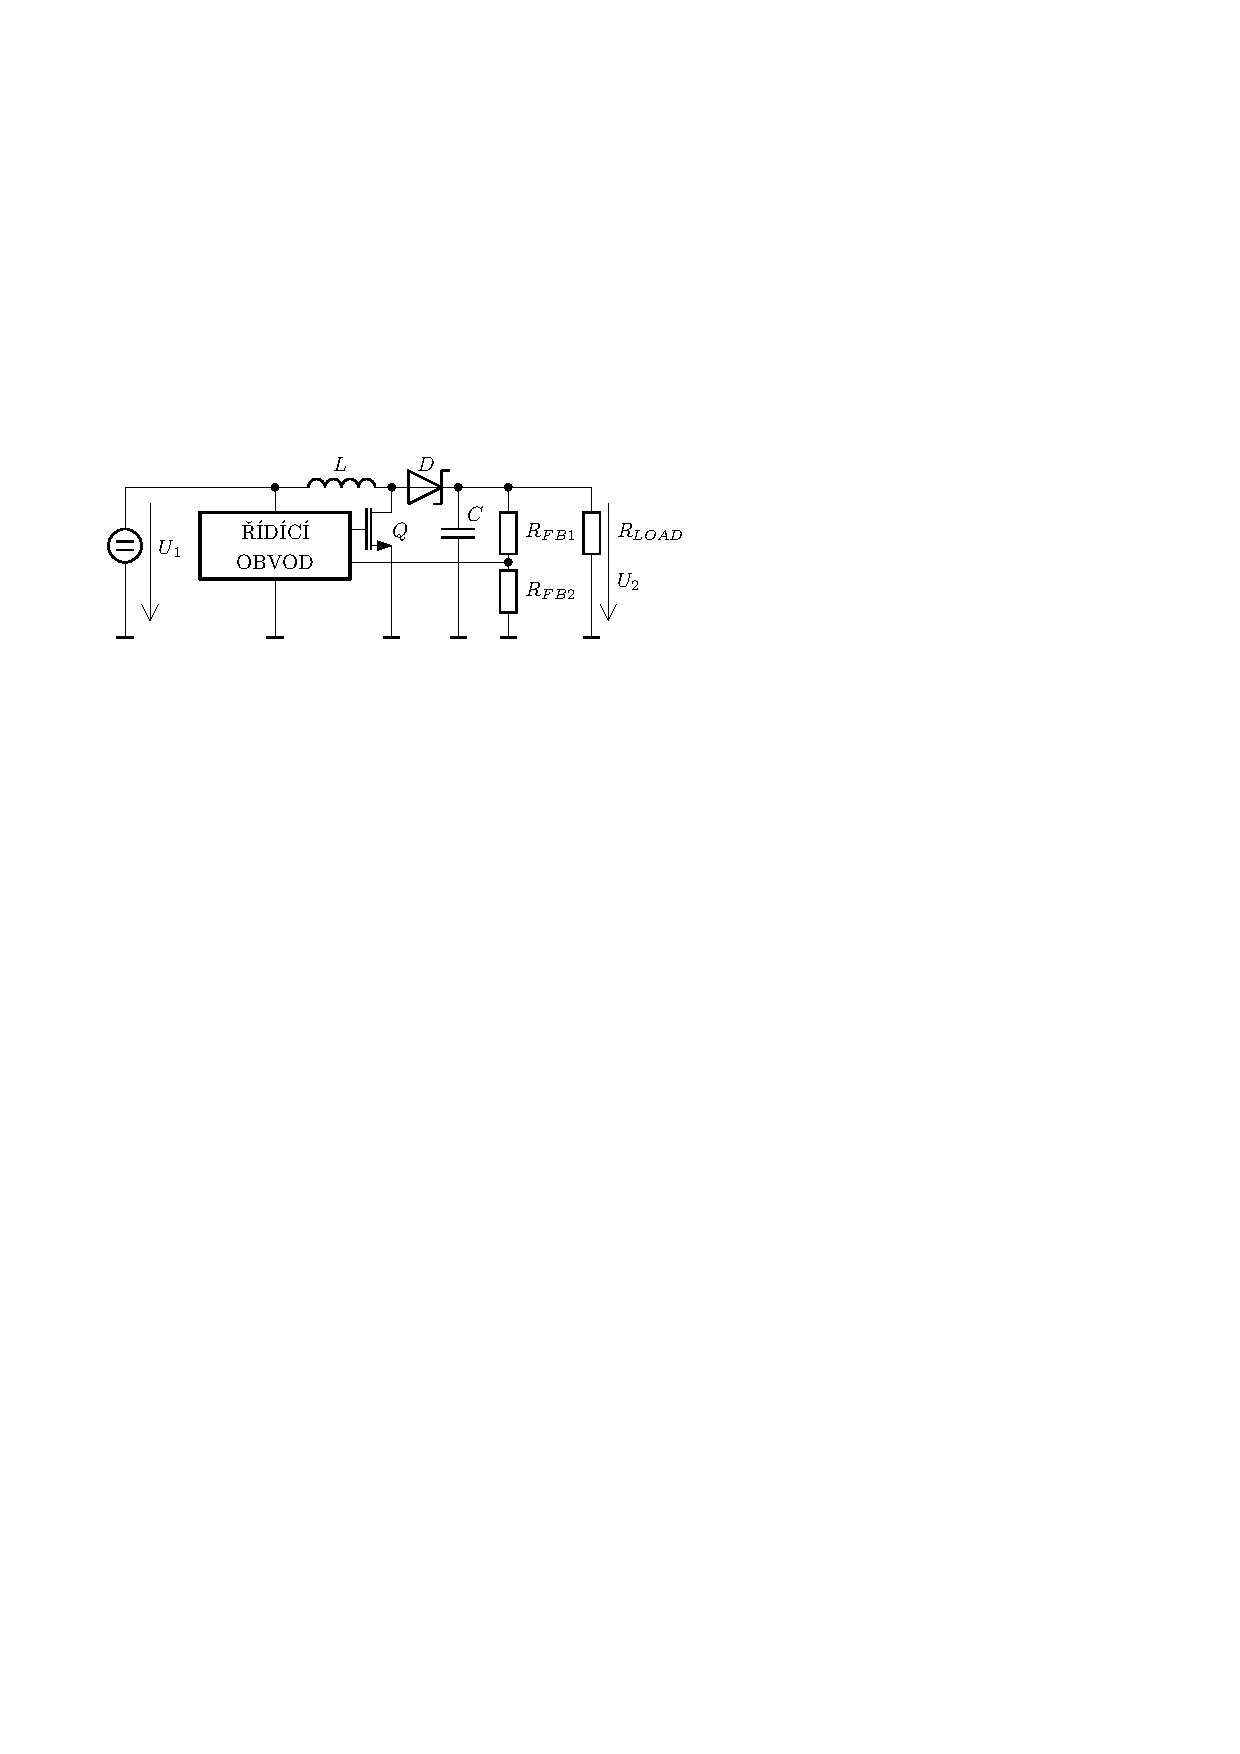
\includegraphics[width=\textwidth]{img/boost}
    \end{center}
    \caption{blokové schéma zvyšujícího měniče}
\end{figure}
Zvyšující měnič, někdy také označovaný jako boost či step up je elektrický obvod, patřící do kategorie spínaných měničů, který z vysokou účinností transformuje vstupní napětí $U_1$ na větší napětí $U_2$. Vstupní i výstupní napětí měniče jsou stejnosměrná.

Měnič obsahuje dva akumulační prvky $L$ a $C$, které slouží k uchování energie a dva prvky aktivní $Q$ a $D$, které plní funkci spínačů. Rezistor $R_{LOAD}$ představuje zátěž.

Pokud je sepnut tranzistor, tak cívka začne akumulovat energii. V tento okamžik je dioda uzavřena, protože napětí na anodě má podprahovou hodnotu. Jakmile dojde k uzavření tranzistoru, tak se otevře dioda a začne se přesouvat akumulovaná energie z cívky do kondenzátoru.

Odvození výstupního napětí zvyšujícího měniče pro ideální spínací prvky:
\begin{eqnarray}
    i_L(t) &=& \dfrac{1}{L} \int u_L(t) \mathrm{d}t \Rightarrow u_L(t) = L \dfrac{\mathrm{d}i_L(t)}{\mathrm{d}t}
    \nonumber\\
    \dfrac{U_1 t_{ON}}{L} &=& \dfrac{(U_2 - U_1) t_{OFF}}{L} \Rightarrow U_1 t_{ON} = (U_2 - U_1) t_{OFF}
    \nonumber\\
    U_1 t_{ON} &=& U_2 t_{OFF} - U_1 t_{OFF} \Rightarrow U_1 T = U_2 t_{OFF}
    \nonumber\\
    U_2 &=& U_1 \dfrac{T}{t_{OFF}} = \underline{\underline{U_1 \dfrac{1}{1-s}}}
    \nonumber
\end{eqnarray}

Kde $t_{OFF}$ je čas po který je tranzistor sepnut, $t_{OFF}$ čas po který je tranzistor rozepnut, $T$ je perioda spínání a $s$ střída spínání.

Ze vztahu je vidět, že napětí $U_2 \geq U_1$. Pokud použijeme reálné součástky, tak tato rovnost neplatí pokud je tranzistor trvale rozepnut, tak napětí $U_2$ bude menší o úbytek na diodě a cívce.

Řídící obvod se snaží udržovat konstantní výstupní napětí, pomocí regulování střídy. Výstupní napětí je monitorováno pomocí zpětné vazby realizované napěťovým děličem. Poměr rezistorů $R_{FB1}$ a $R_{RB2}$ určuje výstupní napětí.

\section{Nabíječka}
TODO

\section{Monitorování náboje}
TODO
